\section{Background}
\label{sec:background}

\begin{figure}[t]
	%\vskip 0.2in
	\begin{center}
		\centerline{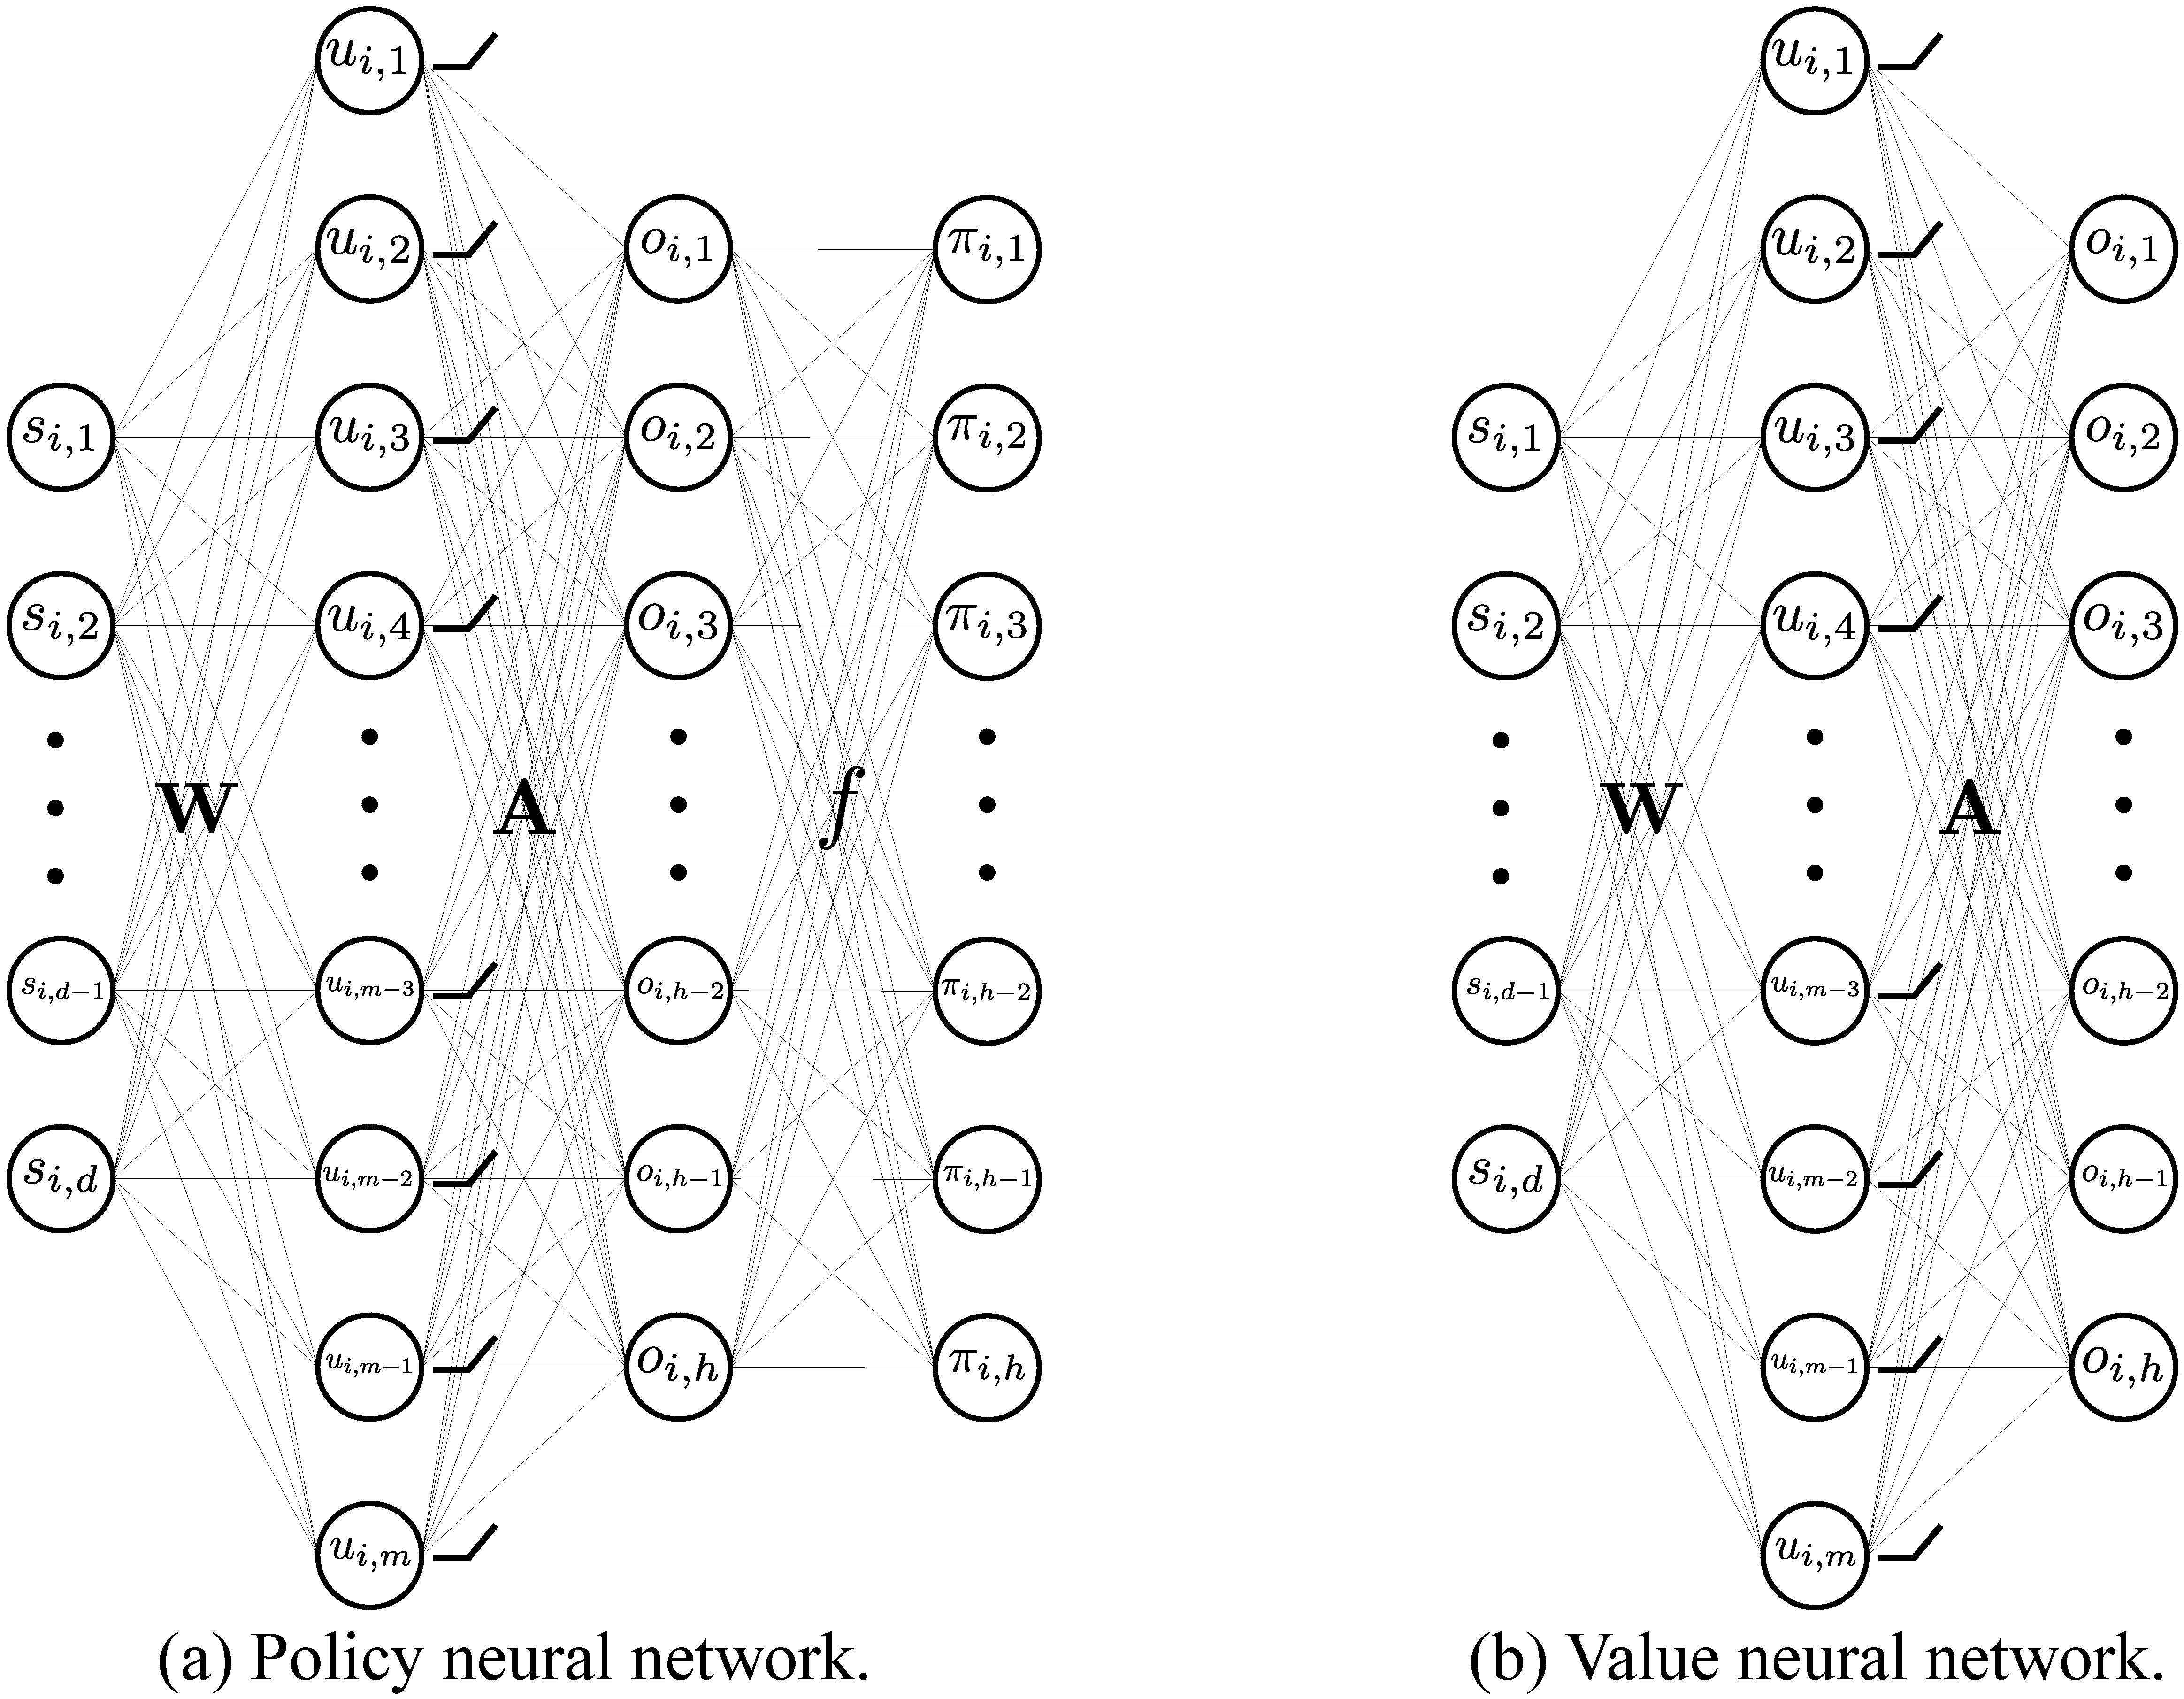
\includegraphics[width=0.55\columnwidth]{nn_policy_value_vertical.pdf}}
		\caption{The structure of the policy neural network and the value neural network.}
		\label{fig:nn_policy_value}
	\end{center}
	\vskip -0.2in
\end{figure}

We mainly focus on the stochastic bandit setting in this paper where the policy or the values of the actions are represented using a 2-layers neural networks.  
However, our results can be easily generalized to many other reinforcement learning settings, e.g. state dependent stochastic bandit settings and episodic MDPs, which will be discussed in \cref{sec:general_settings}.

\subsection{Stochastic Bandit Settings}
\label{subsec:settings}

One can think of that the standard stochastic bandit setting has only $1$ state.  
%At each time step $t$, the agent takes an action $A_t \in [h]$ according to its own strategies $\rvpi_t$, and then it observes a random reward $R\left(A_t\right) \in \sR$, where the mean value of $R\left(A_t\right)$ is $r\left(A_t\right)$. 
%The agent then improves its action selection strategies. 
After $T$ time steps, the performance of the agent's strategy is measured by the (expected) regret,
\begin{equation}
\label{eq:expected_regret}
R_T = \sum\limits_{t=0}^{T-1}{{\rvpi^*}^\top \rvr} - \sE \left[ \sum\limits_{t=0}^{T-1}{  r\left(A_t\right)  } \right] 
%= \sum\limits_{t=0}^{T-1}{{\rvpi^*}^\top \rvr} - \sum\limits_{t=0}^{T-1}{ \sE \left[ r\left(A_t\right) \right] },
\end{equation}
where the expectation is over the randomness of action selection, if the agent is using some stochastic strategies.
Obviously, $\rvpi^*$ is a one-hot vector and by standard calculation, one can show that
\[
R_T = \sum_{t=0}^{T-1} \sum_a \pi_t(a) \Delta(a),
\]
where $\Delta(a) = \max_b r(b)- r(a)$, and  $r(a)$ is the expected reward of the action $a$.
Without loss of generality, in this paper we assume $\rvr \in \left[ 0, 1 \right]^h$.

%\subsubsection{Episodic Markov decision process (MDP) (maybe remove this section)}
%The episodic MDP setting recovers the bandit setting as a special case. The environment randomly select a starting state $\rvs_i^0 \in \sR^d$. At each time step $t$, the agent takes one action $A_t \in [h]$ according to some strategies, and then it observes a reward $R_{i, A_t} \in \sR$ and next state $S_{t+1} \sim \sP\left( \cdot \middle| S_t, A_t \right)$, where $\sP$ is the transition probability matrix and it is unknown to the agent. After such $H$ steps, the agent observes an ending state $S_H$, and the current trajectory terminates. At the next time step, the agent will observe a new starting state $\rvs_i^0$ randomly generated by the environment. Since we use policy gradient method (no value learning), the agent updates its neural network policy weights using the cumulative reward collected after each single trajectory terminates.

%We mainly focus on the standard stochastic bandit setting with $n = 1$, i.e., there is only one state $\rvs_i$. At each time step $t$, the agent takes an action $A_t \in [h]$ according to its own strategies, and then it observes a random reward $R_{i, A_t} \in \sR$, where the mean value of $R_{i, A_t}$ is $r_{i, A_t}$. The agent then uses the reward to improve its action selection strategies. After such $T$ time steps, the performance of the agent's strategy is measured by the (expected) regret,
%\begin{equation}
%\label{eq:expected_regret}
%    \sum\limits_{t=0}^{T-1}{{\rvpi_i^*}^\top \rvr_i} - \sE \left[ \sum\limits_{t=0}^{T-1}{  r_{i, A_t}  } \right] = \sum\limits_{t=0}^{T-1}{{\rvpi_i^*}^\top \rvr_i} - \sum\limits_{t=0}^{T-1}{ \sE \left[ r_{i, A_t} \right] },
%\end{equation}
%where the expectation is over the randomness of action selection, if the agent is using some stochastic strategies.

\subsection{Policy Based and Value Based RL Methods}

Minimizing the regret \cref{eq:expected_regret} is usually formulated as the policy optimization problem, i.e., $\max\limits_{\rvpi \in \Pi}{ \expectation\limits_{ a \sim \rvpi }{ r(a)} }$, where $\Pi$ is the policy constraint. In practice, when $\Pi$ consists of all the $\rvpi\left(\rmW\right)$ represented by the parameter $\rmW$, one can use iterative gradient updates to solve the above expected reward maximization problem. This is known as the policy gradient method.

On the other hand, value based RL methods directly attempt to learn a function to approximate the value of the optimal policy, i.e., $\min\limits_{Q \in \gQ}{ \expectation\limits_{a \sim \rvb}{ \left\| Q(a) - Q^*(a) \right\|_2^2 }}$, where $\rvb$ is a behavior policy that samples actions for the learning. The learned value function induces a policy which acts greedily with respect to the value of each action.

\subsection{Neural Networks as Policy/Value Function Approximations}
\label{subsec:nn_value_policy}
 

%Both the value and the policy neural networks take the state feature  $\rvs_i \in \sR^d$ as the input. Then the networks calculate the hidden node value vector by $u_{i,r} \triangleq \rvw_r^\top \rvs_i$, $\forall r \in [m]$. The logit vector is then calculated by $o_{i,k} \triangleq \rva_k^\top \sigma\left( \rvu_i \right)$, $\forall k \in [h]$, where $\sigma$ is element-wise ReLU activation function. The value neural network outputs the logit vector $\rvo_i$. While the policy neural network output probability is the softmax transform of the logit vector, i.e., $\rvpi_i \triangleq f\left( \rvo_i \right) = f\left( \rmA \sigma\left( \rmW \rvs_i \right) \right)$. 

%The policy neural network defines a family of policies $\rvpi_i \left( \rmW \right)$ parameterized by $\rmW \in \sR^{m \times d}$ given any state $\rvs_i$. Let $\rvpi_i = \rvpi_i \left( \rmW \right)$, the expected loss of the policy neural network can be calculated according to \cref{eq:expected_loss}.

%\paragraph{Initialization of the matrix $\rmA$.} 
Without loss of generality we assume that the networks have the state $\rvs$ as their inputs satisfying $\left\| \rvs \right\|_2 = 1$.
As can be seen later, our algorithm random initializes the weight matrix $\rmA$ and fixes it during learning. 
This is a common strategy when using over-parametrized neural networks, e.g. see \citep{li2018learning,du2018gradientA,du2018gradientB,allen2018convergenceA,allen2018convergenceB}, and it has been empirically verified that there is no impact on the performance of trained neural networks \citep{hoffer2018fix}.
In this paper, each element in $\rmA$ is initialized by $a_{k,r} \sim \unif\left\{-1, +1\right\}$. Some other initializations like $\rva_k \sim \gN(0, \rmI)$ will also work. In the rest of the paper, we denote the policy $\rvpi$ by $\rvpi(\rmW_t)$ to emphasize its parametrization by $\rmW$ at time step $t$. 

%\paragraph{Multi-layered neural networks.} 
We would like to point that our algorithms and results can be extended to general value functions and policies parameterized by multi-layered neural networks resorting to related techniques \citep{allen2018convergenceA,allen2018convergenceB,du2018gradientA}. For the sake of simplicity and conciseness, we only focus on two-layers neural networks in the paper.

%Although there is only one state, i.e., $n = 1$, and $i$ can be omitted without ambiguity, we choose to keep the subscript $i$ here to make the generalization from the standard bandit setting to the many state dependent setting smoother, and our algorithms work for general $n > 1$. For simplicity, we assume $\left\| \rvs_{i} \right\|_2 = 1$, $\forall i \in [n]$.

%In the case of $n > 1$, for each state $\rvs_i$, there is a state dependent policy $\rvpi_i$. And the agent's goal is to learn totally $n$ policies using only one neural network. We assume $\left\| \rvs_{i} -  \rvs_{j} \right\|_2 \ge \delta > 0 , \ \forall i \not= j$, i.e., no duplicated data, and $\left\| \rvs_{i} \right\|_2 = 1, \ \forall i \in [n]$.
